\documentclass[russian,14pt,floatsection,nocolumnsxix]{eskdtext}
% \usepackage[numbertop, numbercenter]{eskdplain}
\usepackage[utf8x]{inputenc}

\usepackage{setspace}
\onehalfspacing % полуторный интервал для всего текста

% - Подключаем шрифты из пакета scalable-cyrfonts-tex
\usepackage{cyrtimes}

% - Отступ красной строки
\setlength{\parindent}{1.25cm}

% - Убирает точку в списке литературы
\makeatletter
\def\@biblabel#1{#1 }

% ограничение для оглавления
%\usepackage{tocvsec2}
\setcounter{tocdepth}{2}

% - Точки для всех пунктов в оглавлении
\renewcommand*{\l@section}{\@dottedtocline{1}{1.5em}{2.3em}}
\renewcommand*{\l@subsection}{\@dottedtocline{1}{1.5em}{2.3em}}
%\renewcommand*{\l@subsubsection}{\@dottedtocline{1}{1.5em}{2.3em}}

% - Для переопределения списков
\renewcommand{\theenumi}{\arabic{enumi}}
\renewcommand{\labelenumi}{\theenumi)}
\makeatother

\usepackage{enumitem}
\setlist{nolistsep, itemsep=0.3cm,parsep=0pt}

% - ГОСТ списка литературы
\bibliographystyle{gost71u2003}

% - Верикальные отступы заголовков 
\ESKDsectSkip{section}{1em}{1em}
\ESKDsectSkip{subsection}{1em}{1em}
\ESKDsectSkip{subsubsection}{1em}{1em}

% - Изменение заголовков
\usepackage{titlesec}
\titleformat{\section}{\normalfont\normalsize\centering}{\thesection}{1.0em}{}
\titleformat{\subsection}{\normalfont\normalsize\centering}{\thesubsection}{1.0em}{}
\titleformat{\subsubsection}{\normalfont\normalsize\centering}{\thesubsubsection}{1.0em}{}
\titleformat{\paragraph}{\normalfont\normalsize\centering}{\theparagraph}{1.0em}{}

% - Оставим место под ТЗ 
%\setcounter{page}{4}

% - Для больших таблиц
\usepackage{longtable}
\usepackage{tabularx}
\renewcommand{\thetable}{\thesection.\arabic{table}}

% - Используем графику в документе
\usepackage{graphicx}
\graphicspath{{images/}}
\renewcommand{\thefigure}{\thesection.\arabic{figure}}

% - Счётчики
\usepackage{eskdtotal}

% - Выравнивание по ширине
\sloppy

% - Разрешить перенос двух последних букв слова
\righthyphenmin=2

% - Оформление списков
\RequirePackage{enumitem}
\renewcommand{\alph}[1]{\asbuk{#1}}
\setlist{nolistsep}
\setitemize[1]{label=--, fullwidth, itemindent=\parindent, 
  listparindent=\parindent}% для дефисного списка
\setitemize[2]{label=--, fullwidth, itemindent=\parindent, 
  listparindent=\parindent, leftmargin=\parindent}
\setenumerate[1]{label=\arabic*), fullwidth, itemindent=\parindent, 
  listparindent=\parindent}% для нумерованного списка
\setenumerate[2]{label=\alph*), fullwidth, itemindent=\parindent, 
  listparindent=\parindent, leftmargin=\parindent}% для списка 2-ой ступени, который будет нумероваться а), б) и т.д.
  
% - Оформляем листинг кода (не использовать комментарии на русском!)
\usepackage{listings}  
\lstset{basicstyle=\ttfamily\scriptsize}
\lstset{extendedchars=\true}

% - выводим текст как есть с размером шрифта scriptsize
\makeatletter
\def\verbatim{\scriptsize\@verbatim \frenchspacing\@vobeyspaces \@xverbatim}
\makeatother

% - Вставка pdf
\usepackage[enable-survey]{pdfpages}

%межстрочный интервал
\usepackage{setspace}
\linespread{1.5}

%фамилии для рамок
\author{\ESKDfontII Поляков И.Ю.}
\ESKDchecker{\ESKDfontII Любутин П.С.}
\ESKDnormContr{\ESKDfontII Майстренко А.В.}
\ESKDapprovedBy{\ESKDfontII Черепанов О.И.}
\ESKDcolumnI{\ESKDfontIII Разработка и тестирование программного обеспечения для оценки деформации поверхности твёрдых тел по серии оптических изображений}
\ESKDcolumnIX{\ESKDfontIII ТУСУР, ФВС, каф.~ЭСАУ, гр.~530}
\ESKDsignature{ЭСАУ.ДР.503390.001.ПЗ}
\begin{document}
\newpage
\ESKDthisStyle{empty}

\begin{center}
Министерство образования и науки Российской Федерации\\
Федеральное государственное бюджетное образовательное учреждение высшего профессионального образования\\
ТОМСКИЙ ГОСУДАРСТВЕННЫЙ УНИВЕРСИТЕТ СИСТЕМ УПРАВЛЕНИЯ И РАДИОЭЛЕКТРОНИКИ (ТУСУР)\\
Кафедра комплексной информационной безопасности электронно-вычислительных систем (ЭСАУ)\\
\end{center}

\hfill
\begin{minipage}[right]{0.4\linewidth}
\begin{singlespace}
 К ЗАЩИТЕ ДОПУСТИТЬ \\
 Заведующий кафедрой ЭСАУ \\
 д.т.н, профессор \\
 \underline{\hspace{2.5cm}}О.И. Черепанов \\
 "\underline{\hspace{1cm}}"\underline{\hspace{3cm}} 2015г.\\
\end{singlespace} 
\end{minipage}


\begin{center}
РАЗРАБОТКА И ТЕСТИРОВАНИЕ ПРОГРАММНОГО ОБЕСПЕЧЕНИЯ ДЛЯ ОЦЕНКИ ДЕФОРМАЦИИ ПОВЕРХНОСТИ ТВЁРДЫХ ТЕЛ ПО СЕРИИ ОПТИЧЕСКИХ ИЗОБРАЖЕНИЙ \\
Дипломная работа \\
по специальности 220301 - Автоматизация технологических процессов и производств\\
\vspace{1.0cm}
\end{center}

СОГЛАСОВАНО
\vspace{0.3cm}
\begin{singlespace}
 \begin{minipage}[left]{0.40\linewidth}
 Консультант по экономике\\
 Доцент кафедры Экономики \\
 канд. экон. наук\\
 \underline{\hspace{2.5cm}}О.П. Полякова \\
 "\underline{\hspace{1cm}}"\underline{\hspace{3cm}} 2015г.\\

 Консультант по безопасности жизнедеятельности\\
 Доцент кафедры РЭТЭМ \\
 канд. хим. наук\\
 \underline{\hspace{2.5cm}}И.А. Екимова\\
 "\underline{\hspace{1cm}}"\underline{\hspace{3cm}} 2015г.\\
 \end{minipage}
 \hfill
 \begin{minipage}[left]{0.5\linewidth}
  \vspace{0.64cm}
 Студент гр. 530 \\
 кафедры ЭСАУ \\
 \underline{\hspace{2.5cm}}И.Ю. Поляков \\
 "\underline{\hspace{1cm}}"\underline{\hspace{3cm}} 2015г.\\
 \vspace{0.59cm}\\ 
 Руководитель\\
 Мл. н. с. лаборатории полимерных композитных материалов
 ИФПМ СО РАН \\
 канд. техн. наук\\
 \underline{\hspace{2.5cm}}П.С. Любутин \\
 "\underline{\hspace{1cm}}"\underline{\hspace{3cm}} 2015г.\\
 \end{minipage}
\end{singlespace}

\vfill
\begin{center}
Томск -- 2015
\end{center}
\newpage
\ESKDthisStyle{empty}
\paragraph{\hfill Реферат \hfill}
Выпускная квалификационная работа \ESKDtotal{page} с., \ESKDtotal{figure} рис., \ESKDtotal{table} табл., \ESKDtotal{bibitem} источников, \ESKDtotal{appendix} прил.


ПОЛЕ ВЕКТОРОВ СМЕЩЕНИЙ, КОМПОНЕНТЫ ДЕФОРМАЦИИ, СУБПИКСЕЛЬНАЯ ТОЧНОСТЬ

Целью настоящей работы является разработка программного обеспечения (ПО) для оценки деформаций поверхностей твёрдых тел, а также проведение исследований алгоритмов и методов как на модельных, так и на реальных оптических изображениях.

В работе исследовано влияние метода интерполяции изображений с субпиксельной точностью с использованием итеративного подхода на расчёт оптического потока(векторного поля).

Проект выполнен с использованием следующих средств разработки: языка программирования C++(Qt), среды разработки QtCreator 3, Sublime 3. Система контроля версий git.

Программное обеспечение, разработанное в ходе данной работы, представлено в приложении.

Отчёт выполнен согласно ОС ТУСУР 01-2013 при помощи текстового процессора \LaTeX.
\newpage
\ESKDthisStyle{empty}
\paragraph{\hfill The abstract \hfill}
Diploma work contains \ESKDtotal{page} pages, \ESKDtotal{figure} pictures, \ESKDtotal{table} tables, \ESKDtotal{bibitem} sources, \ESKDtotal{appendix} appendix, 5 sheets of a graphic material.

FIELD DISPLACEMENT VECTOR, STRAIN COMPONENTS, SUB-PIXEL ACCURACY

The aim of this work is the development of software (software) to evaluate the deformation of surfaces of solids, as well as research methods and algorithms on model, and the real optical images.

The influence of the method of interpolation image with sub-pixel precision using an iterative approach to the calculation of the optical flow (vector field).


The project was implemented using the following development tools: the programming language C ++ (Qt), development environment QtCreator 3, Sublime 3. A version control system git.

The software, developed in the course of this work, presented in the annex.

The report is made in accordance with the OS TUSUR 01-2013 using a word processor \LaTeX.
\newpage
\ESKDthisStyle{empty}

\begin{center}
 Министерство образования и науки Российской Федерации\\
 Федеральное государственное бюджетное образовательное учреждение высшего профессионального образования\\
 ТОМСКИЙ ГОСУДАРСТВЕННЫЙ УНИВЕРСИТЕТ СИСТЕМ УПРАВЛЕНИЯ И РАДИОЭЛЕКТРОНИКИ (ТУСУР)\\
 Кафедра электронных средств автоматизации и управления (ЭСАУ)\\
\end{center}

\begin{flushright}
 \begin{minipage}{0.4\textwidth}
  УТВЕРЖДАЮ \\
  зав. каф. ЭСАУ \\
  \underline{\hspace{2.5cm}}О.И. Черепанов \\
  "\underline{\hspace{1cm}}"\underline{\hspace{3cm}} 2015г.
 \end{minipage}
\end{flushright}

\vspace{1cm}

\paragraph*{\hfill ЗАДАНИЕ \hfill}

на дипломную работу студенту Полякову Игорю Юрьевичу группы 530, факультета вычислительных систем.

1. Тема работы: Разработка и тестирование программного обеспечения для оценки деформации поверхности твёрдых тел по серии оптических изображений.

2. Срок сдачи студентом законченной работы: "\underline{\hspace{1cm}}"\underline{\hspace{3cm}} 2015г.

3. Исходные данные к работе:

\begin{itemize}
 \item Программное обеспечение для оценки деформации ``Deformation Analysis'';
 \item Дифференциальный алгоритм Лукаса−Канаде.
\end{itemize}
\newpage
4. Содержание расчётно-пояснительной записки (перечень подлежащих разработке вопросов):

\begin{itemize}
 \item введение;
 \item описание алгоритмов;
 \item проектирование программного обеспечения;
 \item тестирование;
 \item заключение.
\end{itemize}

5. Перечень графического материала:

\begin{itemize}
 \item презентация.
\end{itemize}

6. Консультанты по работе

\begin{itemize}
  \item консультант по экономике: доцент кафедры экономики, кандидат \\ экономических наук \\
  \begin{singlespace}
 О.П. Полякова\hfill \underline{\hspace{6cm}} \\
 \begin{flushright} "\underline{\hspace{1cm}}"\underline{\hspace{3cm}} 2015г. \end{flushright}
 \end{singlespace}
 \item консультант по вопросам охраны труда: доцент кафедры РЭТЭМ, кандидат химических наук\\
 \begin{singlespace}
 И.А. Екимова \hfill \underline{\hspace{6cm}} \\
 \begin{flushright} "\underline{\hspace{1cm}}"\underline{\hspace{3cm}} 2015г. \end{flushright}
 \end{singlespace}
\end{itemize}

Задание выдано:

Руководитель: младший научный сотрудник ИФПМ СО РАН, кандидат технических наук \\
\begin{singlespace}
П.С. Любутин \hfill \underline{\hspace{6cm}} \\
\begin{flushright} "\underline{\hspace{1cm}}"\underline{\hspace{3cm}} 2015г. \end{flushright}
\end{singlespace}

Задание принято к исполнению:

\begin{singlespace}
студент И.Ю. Поляков \hfill \underline{\hspace{6cm}} \\
\begin{flushright} "\underline{\hspace{1cm}}"\underline{\hspace{3cm}} 2015г. \end{flushright}
\end{singlespace}
\newpage
\ESKDstyle{formIIab}
\ESKDthisStyle{formII}
\renewcommand\contentsname{\hfill Содержание \hfill}
\tableofcontents
\setcounter{figure}{0}
\newpage
\section*{Введение}
\addcontentsline{toc}{section}{Введение}

XXXXXXXXXXXXXXX
\newpage
\section{Описание алгоритмов и методов для решения задачи}
Все современные дифференциальные алгоритмы слежения за особенностями опираются на работу 1981 году Лукаса и Канаде \cite{Lucas1981}. В 1991 году математическая формулировка этого алгоритма была изменена, и стала основой для всех последующих обобщений с учётом аффинных искажений окрестности и освещённости. Путём замены соответствующих переменных на константы любой из них превращается в обычный алгоритм Лукаса−Канаде \cite{lk_jou}.
\subsection{Описание дифференциального алгоритма определения оптического потока Лукаса−Канаде}
\label{subsec:lycas_kanade_81}
В основе всех дальнейших рассуждений лежит одно очень важное и не очень справедливое предположение: Предположим, что значения пикселей переходят из одного кадра в следующий без изменений. Таким образом, мы делаем допущение, что пиксели, относящиеся к одному и тому же объекту, могут сместиться в какую либо сторону, но их значение останется неизменным. Конечно же это предположение имеет мало общего с реальностью, потому что от кадра к кадру могут меняться глобальные условия освещения и освещённость самого движущегося объекта. Масса проблем связана с этим допущением, но, как ни странно, вопреки всему оно достаточно хорошо работает на практике. На математическом языке это допущение можно записать так:
\numberwithin{equation}{section}
\label{eq:f_0}
\begin{equation}
I(x,y,t)=I(x+u_x,y+u_y,t+1)
\end{equation}

где $I$ — это функция яркости пикселей от положения на кадре и времени. Другими словами $x$ и $y$ — это координаты пикселя в плоскости кадра, и — это смещение, а $t$ — это номер кадра в последовательности. Условимся, что между двумя соседними кадрами проходит единичный отрезок времени.
\subsubsection{Одномерный случай алгоритма}

\begin{figure}[ht]
\center{\includegraphics[width=0.4\linewidth]{math_1}}
\caption{Одномерный сдвиг яркостей}
\label{pic:math_1}
\end{figure}

Для начала рассмотрим одномерный случай. Рассмотрим представленные на рисунке \ref{pic:math_1} два одномерных кадра размером 1х20 пикселей. На рисунке \ref{pic:math_1} кадр $f_2$ смещено вправо на 4 пикселя. Именно это смещение необходимо найти. Для этого представим эти же кадры в виде функций (рисунок \ref{pic:math_2}). На входе позиция пикселя, на выходе — его интенсивность. В таком представление искомое смещение ($d$) видно еще более наглядно. В соответствии с нашим предположением,$f_2$ это просто смещённая $f_1$, то есть можно сказать, что:

\numberwithin{equation}{section}
\label{eq:f_2}
\begin{equation}
f_2(x)=f_1(x-d)
\end{equation}

\begin{figure}[ht]
\center{\includegraphics[width=0.4\linewidth]{math_2}}
\caption{Функция зависимости интенсивности от позиции пикселя}
\label{pic:math_2}
\end{figure}

Обратите внимание, что $f_1$ и $f_2$ при желании можно записать и в общем виде: $f_1(x)=I(x,y,t)$ $f_2(x)=I(x,y,t)$ ; где $y$ и $t$ зафиксированы и равны нулю.

Для каждой координаты нам известны значения и в этой точке, кроме того мы можем вычислить их производные. Свяжем известные значения со смещением $d$. Для этого запишем разложение в ряд Тейлора для $f_1(x-d)$:
$$f_1(x-d)=f_1(x)-df^{'}_1(x)+O(d^2f^{''}_1)$$

Сделаем второе важное предположение: Предположим, что достаточно хорошо аппроксимируется первой производной. Сделав это предположение, отбросим всё что после первой производной:
$$f_1(x-d)=f_1(x)-df_1^{'}(x)$$

Насколько это корректно? В общем—то не очень, тут мы теряем в точности, если только наша функция/изображение не строго линейна, как в нашем искусственном примере. Зато это существенно упрощает метод, а для достижения требуемой точности можно сделать последовательное приближение, которе мы рассмотрим позже.

Мы почти у цели. Смещение $d$ — это наша искомая величина. Исходя из \ref{eq:f_2}, сделаем замену:$f_2(x)=f_1(x)-df_1^{'}(x)$
откуда выведем $d = \dfrac{f_1(x)-f_2}{f_1^{'}(x)}$
\subsubsection{Двумерный случай алгоритма}

Теперь перейдём от одномерного случая к двумерному. Запишем разложение в ряд Тейлора для \ref{eq:f_0} и сразу отбросим все старшие производные. Вместо первой производной появляется градиент:
$$I(x+u_x,y+u_y,t+1)=I(x,y,t)+\overrightarrow{u} \nabla I(x,y,t)$$
где $\overrightarrow{u} = \begin{bmatrix}
u_x\\
u_y
\end{bmatrix} $ — вектор смещения.
В соответствии со сделанным допущением \ref{eq:f_0}. Перепишем:
$$I(x,y,t)-I(x_x,y_y,t+1) + \overrightarrow{u} \nabla I(x,y,t) = 0$$
Поскольку между двумя кадрами проходит единичный интервал времени, то можно сказать, что $I(x,y,t)-I(x,y,t+1)$ есть не что иное, как производная по времени.
Заменим:
$$\frac{\partial I(x,y,t)}{\partial t} + \overrightarrow{u} \nabla I(x,y,t) = 0$$
Перепишем ещё раз, раскрыв градиент:
$$\frac{\partial I(x,y,t)}{\partial t} + u_x\frac{\partial I(x,y,t)}{\partial x} + u_y\frac{\partial I(x,y,t)}{\partial y} = 0$$

Мы получили уравнение, которое говорит нам о том, что сумма частных производных должны быть равна нулю. Проблема только в том, что уравнение у нас одно, а неизвестных в нем два: $u_x$ и $u_y$. На этом моменте начинается полет фантазии и разнообразие подходов.

Сделаем третье предположение: Предположим, что смещение пикселей между двумя кадрами невелико. Рассмотрим пиксель $p$, тогда, по алгоритму Лукаса — Канаде, оптический поток должен быть одинаков для всех пикселей, находящихся в окне с центром в $p$. А именно, вектор оптического потока $u_x$ и $u_y$ в точке $p$ должен быть решением системы уравнений. Очевидно, что в общем случае система не имеет решения, поэтому будем искать такие $u_x$ и $u_y$, которые минимизируют ошибку:
$$
\begin{cases}
I_x(q_1) V_x + I_y (q_1) V_y = -I_t(q_1)\\
I_x(q_2) V_x + I_y (q_2) V_y = -I_t(q_2)\\
...\\
I_x(q_n) V_x + I_y (q_n) V_y = -I_t(q_n)\\
\end{cases}
$$
где $q_1,q_2,\dots,q_n$ — пиксели внутри окна
$I_x(q_i),I_y(q_i),I_t(q_i)$ — частные производные изображения $I$ по координатам $x$, $y$ и времени $t$, вычисленные в точке $q_i$.
Это уравнение может быть записано в матричной форме:
$$A v = b$$

$$A = \begin{bmatrix}
I_x(q_1) && I_y(q_1) \\
I_x(q_2) && I_y(q_2) \\
\vdots && \vdots \\
I_x(q_n) && I_y(q_n)
\end{bmatrix},
\quad\quad
v =
\begin{bmatrix}
V_x\\
V_y
\end{bmatrix},
\quad\quad
b =
\begin{bmatrix}
-I_t(q_1)\\
-I_t(q_2)\\
\vdots \\
-I_t(q_n)
\end{bmatrix} $$
Полученную переопределенную систему решаем с помощью метода наименьших квадратов. Таким образом, получается система уравнений $2 \cdot 2$:
$$A^T A v=A^T b$$
откуда
$$\mathrm{v}=(A^T A)^{-1}A^T b$$
где $A^T$ — транспонированная матрица $A$. Получаем:
$$\begin{bmatrix} V_x\\[10pt] V_y \end{bmatrix} = \begin{bmatrix} \sum_i I_x(q_i)^2 & \sum_i I_x(q_i)I_y(q_i) \\[10pt] \sum_i I_x(q_i)I_y(q_i) & \sum_i I_y(q_i)^2 \end{bmatrix}^{-1} \begin{bmatrix} -\sum_i I_x(q_i)I_t(q_i) \\[10pt] -\sum_i I_y(q_i)I_t(q_i) \end{bmatrix}$$

Вот собственно и все. Мы знаем приблизительное смещение пикселей между двумя соседними кадрами.

Поскольку в нахождении смещения каждого пикселя участвуют также соседние с ним пиксели, при реализации данного метода целесообразно предварительно посчитать производные кадра по горизонтали и вертикали.
\subsubsection{Итеративный подход и субпиксельная точность} %Недостатки метода}

Описанный выше метод основан на трёх значительных допущениях, которые с одной стороны дают нам принципиальную возможность определить оптический поток, но с другой стороны вносят погрешность. 
\begin{figure}[ht]
\center{\includegraphics[width=0.4\linewidth]{math_3}}
\caption{Функция зависимости интенсивности от позиции пикселя}
\label{pic:math_3}
\end{figure}

Одно из допущений нужно нам только для упрощения метода, и с его последствиями мы можем бороться. Мы предполагали, что для аппроксимации смещения нам будет достаточно первой производной. В общем случае это конечно же не так (рисунок \ref{pic:math_3}). 

Для достижение требуемой точности смещение для каждой пары кадров (назовём их $F_i$ и $F_{i+1}$) можно вычислять итеративно. В литературе это называется искажением (warping). На практике это означает, что, вычислив смещения на первой итерации, мы перемещаем каждый пиксель кадра в противоположную сторону так, чтобы это смещение компенсировать.

На следующей итерации вместо исходного кадра $F_{i+1}$ мы будем использовать его искажённый вариант $F_{i+1}^1$. И так далее, пока на очередной итерации все полученные смещения не окажутся меньше заданного порогового значения. Итоговое смещение для каждого конкретного пикселя мы получаем как сумму его смещений на всех итерациях. 
\begin{figure}[ht]
\center{\includegraphics[width=0.4\linewidth]{grid_}}
\caption{Окрестность с субпиксельной точностью}
\label{pic:grid}
\end{figure}

Возникает одна проблема, искажённая область дискретна и состоит из пикселей. Мы не можем сместить область на значение $x,y$, если оно лежит в интервале $0< |x,y| < 1$. Решением этой проблемы является — интерполяция или субпиксельная точность (рисунок \ref{pic:grid}).

В работе описывающей Пирамидальную версию алгоритма \cite{Bouguet2000}, которая подробнее описана в разделе \ref{subsec:pyramid}, предлагалось использовать билинейную интерполяцию однако, хотелось бы попробовать другие способы интерполяции, и посмотреть на выходные результаты.

Методы интерполяции использованные для разработки и последующего тестирования:
\begin{itemize}
\item Билинейная
\item Бикубическая
\item Б-сплайн
\end{itemize}
 $http://algolist.manual.ru/graphics/3dfaq/articles/71.php$

По своей природе данный метод является локальным, то есть при определении смещения конкретного пикселя принимается во внимание только область вокруг этого пикселя — локальная окрестность. Как следствие, невозможно определить смещения внутри достаточно больших (больше размера локальной окрестности) равномерно окрашенных участков кадра. К счастью на реальных кадрах такие участки встречаются не часто, но эта особенность все же вносит дополнительное отклонение от истинного смещения.

Если интервал времени между кадрами принять за 1, получается следующий алгоритм:
$$\begin{cases} d_k = 0 &\mbox{if } k = 0 \\
d_{k+1}=d_k + C^{-1} \sum_W \left[ (I(x,t) - I(x+d_k,t + 1)) \nabla I (x,t) \right] & \mbox{if } k > 0 \end{cases}
$$
Таким образом, этот алгоритм слежения фактически является поиском точки, в которой достигается минимум некоторой функции, методом градиентного спуска. Во время каждой итерации мы сдвигаемся вдоль направления градиента изображения в текущей точке.
\subsubsection{Учёт аффинных преобразований}
Перемещение объекта на входящем видео потоке, описанное в разделе \ref{subsec:lycas_kanade_81}, одно из простейших видов движения. Существуют более сложные: сжатие, увлечение, вращение и т.д. По сути это преобразование плоскостей, называемое аффинным. При условии:
\begin{itemize}
\item[оно взаимно однозначно;]
\item[образом любой прямой является прямая.]
\end{itemize}

Алгоритм с учётом аффинных искажений хорошо описан в работе Ши Томаси канаде в 1994 году \cite{shi_tom_lyk}. Движение пикселей окна описывается в виде $Ax + d$, где $A$ — матрица $(2 \cdot 2)$, $а d$ — смещение $(2 \cdot 1)$.

Задача слежения за особенностью сводится к проблеме проблема определения параметров движения и искажения окна особенности, при которой минимизируется разность:
$$r=\iint_W [J(\Delta x+d)-I(x)]^2$$
где $W$ — окно особенности, а $w$ — весовая функция (может использовать, а может и быть равна 1 во всем окне), $J(x)$ и $I(x)$ — два изображения.

Выражение дифференцируется относительно параметров движения, и производная приравнивается к 0. Затем система линеаризуется с помощью разложения функции изображения в ряд Тейлора:
$$J(\Delta x+d)= J(x)+g^T(u)$$

Это даст нам линейную $6 \cdot 6$ систему:
$$Tz=a$$
, где в векторе $z$ объединены все искомые параметры:

$$z^T=\begin{bmatrix}
 d_{xx} & d_{yx} & d_{xy} & d_{yy} & d_x & d_y
\end{bmatrix}$$
Вектор ошибки a записывается в виде:
$$a=\iint_W [I(x)-J(x)]\begin{bmatrix}
xg_x\\
xg_y\\
yg_x\\
yg_y\\
g_x\\
g_y
\end{bmatrix}\omega dx$$
А матрицу размерности $6 \cdot 6$ $T$ можно представить следующим образом:
$$T=\iint_W [I(x)-J(x)]\begin{bmatrix}
U & V\\
V^T & Z
\end{bmatrix}\omega dx$$

$$U=\begin{bmatrix}
x^3 g^3_x & x^3 g_x g_y & x y g^3_x & x y g_x g_y \\
x^3g_xg_y & x^3g^3_y & xyg_xg_y & xyg^3_x \\
xyg^3_x & xyg_xg_y & y^3g^3_x & y^3g_xg_y \\
xyg_xg_y & xyg^3_y & y^3g_xg_y & y^3g^3_y
\end{bmatrix}$$

$$V^T=\begin{bmatrix}
xg^3_x & xg_xg_y & yg^3_x & yg_xg_y \\
xg_xg_y & xg^3_y & yg_xg_y & yg^3_y
\end{bmatrix}$$

$$Z=\begin{bmatrix}
g^3_x & g_xg_y \\
g_xg_y & g^3_y
\end{bmatrix}$$

Полученная система решается также итеративно по методу Ньютона—Рафсона.

Если движение считается не аффинным, а просто смещением, то первые четыре элемента искомого вектора $z$ обращаются в 0, и значимыми остаются только последние два. Алгоритм превращается в алгоритм Tomasi—Kanade.
\subsubsection{Пирамидальная версия алгоритма}
\label{subsec:pyramid}
Пирамидальная версия или иерархический метод. В данном алгоритме важным является нахождение хорошего начального приближения для вектора скорости. Для этого обычно применяют пирамидальную версию алгоритма. Ее идея заключается в том, что наряду с исходной парой изображений ( f; g ) рассматривают эти же изображения сжатые в два раза ( f 2 ; g 2 ) , в четыре ( f 4 ; g 4 ) и т.д. ( пирамида ). Вектора скорости находят сначала на самом верхнем уровне пирамиды и затем спускаются вниз этаж за этажом. На самом верхнем уровне в качестве начального приближения берут нулевой вектор. На нижних уровнях за начальное приближение берут удвоенную скорость, полученную на предыдущем шаге. Все это вместе взятое обеспечивает хорошее сочетание скорости, точности и устойчивости алгоритма нахождения межкадрового движения в виде сдвигов \cite{Bouguet2000}.

Каждое изображение последовательности, за исключением первого, получается как свёртка предыдущего изображения со следующим фильтром:
(рис. \ref{pic:pyramid}).
Пирамидальный алгоритм Лукаса — Канаде для поиска потока в точке $(x_0,y_0)$.
\begin{enumerate}
\item По каждому из двух данных изображениям строится пирамида изображений
\item Для $i$ – го изображения пирамиды по первому и второму изображениям применяется классический KLT метод, с вектором начального приближения $2 \cdot d_{i+1}$, где $d_{i+1}$ – вектор потока, полученный на предыдущем уровне пирамиды.
\end{enumerate}
Для самого первого уровня этот вектор принимается равным (0,0).

\begin{figure}[ht]
\center{\includegraphics[width=0.6\linewidth]{pyramid}}
\caption{Пример пирамиды Гаусса}
\label{pic:pyramid}
\end{figure}

\subsection{Оценка деформации}
Деформация — изменение размеров и формы твёрдого тела под действием внешних сил (нагрузок) или каких—либо действий (например, температуры, электрических или магнитных полей).

При деформации точки твёрдого тела меняют своё положение. Точка с радиус—вектором $r$ при деформации имеет новое положение $r^{\prime}$, то есть осуществит перемещения $u = r^{\prime} — r$. Поле перемещений является одной из характеристик деформации, но оно неудобное для математического описания, поскольку, например, при удлинение стержня точки у его начала смещаются совсем мало, а в конце — довольно значительно. Гораздо важнее то, насколько точка тела сместилась относительно соседней. Поэтому деформацию математически удобнее описывать производными от перемещения, которые образуют тензор, получивший название тензора деформации.

Виды деформаций
\subsubsection{Линейная деформация Одноосный случай}

Проявляется в растяжении—сжатии стержня вдоль его оси. Если выбрать в ненагруженном стержни два сечения, расположенных на определённом расстоянии и приложить к нему внешние силы, то расстояние между сечениями изменится.

Линейная деформация $\varepsilon$ в произвольной точке тела является границей отношение прироста длины $\delta L$ к исходной длины $L$, когда сама длина стремится к нулю.

\[ \varepsilon = \lim_{L \to 0} \frac{{\delta} {L}} {L} \]

То есть при определении деформации в точке рассматриваются изменения в ее непосредственном окрестности.
Общий случай

Для произвольного тела, испытывающего произвольного деформирования значение линейных деформаций может отличаться в зависимости от направления, в котором они рассматриваются. В этом случае линейные деформации рассматриваются в проекциях на оси декартовых координат. Тогда деформация отрезка AB, лежит на оси x и точка B которая после деформации переместится в т. B 'запишется как:

\[ \varepsilon_x = \lim_{B \to A} {{| AB '| - | AB |} \over {| AB |}} \]

Проведя подобный анализ для осей $y$ и $z$ можно получить соответственно $\varepsilon_y$ и $\varepsilon_z$.

Имея это поле перемещений $\ overrightarrow u$ (компоненты вектора перемещений для всех точек тела) можно записать в общем линейные деформации как:

\[\varepsilon_x = {{\partial u_x} \over {\partial x}}; \varepsilon_y = {{\partial u_y} \over {\partial y}}; \varepsilon_z = {{\partial u_z} \over {\partial z}} \]

\subsubsection{Деформация сдвига}

Аналогично оценивается деформация сдвига (изменение углов) в непосредственном окрестности точки. Угловая деформация $\gamma$ является границей изменения угла между двумя произвольно выбранными отрезками в теле при приложении нагрузки, когда длины этих отрезков стремятся к нулю. Имея это поле перемещений как и выше можно записать:

\[\gamma_{xy} = {{\partial u_x} \over {\partial y}} + {{\partial u_y} \over {\partial x}}; \gamma_{yz} = {{\partial u_y} \over {\partial z}} + {{\partial u_z} \over {\partial y}}; \gamma_{xz} = {{\partial u_x} \over {\partial z}} + {{\partial u_z} \over {\partial x}} \]

\subsubsection{Объёмная деформация}

Хотя деформации линейные $\varepsilon$ и угловые $\gamma$ полностью описывают деформированное состояние тела, является иногда целесообразным характеризовать другие виды деформаций, как, например, объёмная деформация, выступает как мера изменения объёма тела. Из определения объёмная деформация то:

\[\vartheta = \lim_{V^{(0)} \to 0} {V - V^{(0)} \over {V^{(0)}}} \]

где: V (0) — начальный объем, V — конечное значение объёма.

Можно доказать, что в декартовой системе координат:

\[ \vartheta = \varepsilon_x + \varepsilon_y + \varepsilon_z \]

Тензорный запись деформации

Используя единые обозначения для обоих типов деформации можно записать деформации в виде тензора деформации:

\[  \varepsilon_{ij} = {1 \ over 2} \left ({\nabla_i u_j + \nabla_j u_i} \right), \]

или в тензорном виде:

\[  \varepsilon = {1 \over 2} (\vec {\nabla} \vec {u} + (\ vec {\nabla} \vec {u}) ^ T) \]

Из сравнения тензорного записи с тардицийним для декартовой системы координат можно получить:

\[ \varepsilon_{ij} = \left [{\begin {matrix} {\varepsilon_x} & {{{\gamma _{xy}} \over 2}} & {{{\gamma_{xz}} \over 2}} \\ {{{\gamma_{xy}} \over 2}} & {\varepsilon_y} & {{{\gamma_{yz}} \over 2}} \\ {{{\gamma_{xz}} \over 2}} & {{{\gamma_{yz}} \over 2}} & {\varepsilon_z} \end{matrix}} \right] \]

Объёмная деформация: \[ \vartheta = \varepsilon_{ij} g^{ij} \]

где: $g_{ij}$ — контравариантный метрический тензор.
Типичные виды деформаций

Самые распространённые виды деформации, которые рассматриваются сопротивлением материалов — изгиб, сдвиг (срез), кручение, растяжение—сжатие.

Компоненты рассчитываются путём численного дифференцирования полученного поля смещений. Выражения для продольной $\varepsilon_{xx}$, поперечной $\varepsilon_{yy}$, сдвиговой $\varepsilon_{xy}$ и поворотной $\omega_z$ компонент тензора дисторсии:

$$\varepsilon_{xx}= \frac{\mathrm{d} U_x}{\mathrm{d} x},\varepsilon_{yy}= \frac{\mathrm{d} U_y}{\mathrm{d} y},\varepsilon_{xy}=\frac{1}{2}(\frac{\mathrm{d} U_x}{\mathrm{d} y} + \frac{\mathrm{d} U_y}{\mathrm{d} x}),\omega_z=\frac{1}{2}(\frac{\mathrm{d} U_y}{\mathrm{d} x} - \frac{\mathrm{d} U_x}{\mathrm{d} y})$$

Также выражение для интенсивности деформации сдвига $\gamma_i$

$$\gamma_i = \sqrt\frac{2}{3}\sqrt{(\varepsilon_{xx}-\varepsilon_{xx})^2+\varepsilon_{yy}^2+\varepsilon_{xx}^2 + \frac{3}{2}\varepsilon_{xy}^2}$$
\newpage
\section{Конструкторско-технологическая часть}
\subsection {Программная платформа и язык программирования}
Для решения поставленной задачи необходимо использовать функциональную, эффективную и удобную платформу для разработки. В качестве такой платформы была выбрана среда разработки Qt Creator.
Qt - это кросс-платформенная библиотека C++ классов для создания графических пользовательских интерфейсов (GUI) от фирмы Digia. Эта библиотека полностью объектно-ориентированная, что обеспечивает лёгкое расширение возможностей и создание новых компонентов. Ко всему прочему, она поддерживает огромнейшее количество платформ.

Qt позволяет запускать написанное с его помощью ПО в большинстве современных операционных систем путём простой компиляции программы для каждой ОС без изменения исходного кода. Включает в себя все основные классы, которые могут потребоваться при разработке прикладного программного обеспечения, начиная от элементов графического интерфейса и заканчивая классами для работы с сетью, базами данных и XML. Qt является полностью объектно-ориентированным, легко расширяемым и поддерживающим технику компонентного программирования.

Список использованных классов фреймворка Qt:
\begin{itemize}
\item QDebug;
\item QDir;
\item QFile;
\item QTextStream;
\item QSrting;
\item *QImage.
\end{itemize}

Класс QDebug обеспечивает выходной поток для отладочной информации.

Класс QDir обеспечивает доступ к структуре каталогов и их содержимого.

Класс QFile предоставляет интерфейс для чтения и записи файлов.

Класс QTextStream предоставляет удобный интерфейс для чтения и записи текста.

Класс QString обеспечивает строку символов Unicode.

Класс QImage предоставляет аппаратно-независимую работу с изображениями, даёт прямой доступ к данным каждого пикселя, и может быть использован в качестве устройства рисования. На ранних стадиях создание ПО это класс использовался в качестве основного инструмента для работы с изображениями, но впоследствии при переходе на основные модули библиотеки DV стал использовался объект Data2Db, и методы работы с ними.

Список стандартных библиотек используемых в проекте:

\begin{itemize}
\item getopt.h;
\item iostream;
\item math.h;
\item stdlib.h;
\item vector.
\end{itemize}

getopt библиотечная функция, специально разработанная для того чтобы облегчить обработку входных команд. 

iostream заголовочный файл с классами, функциями и переменными для организации ввода-вывода в языке программирования C++. Он включён в стандартную библиотеку C++. Название образовано от Input/Output Stream («поток ввода-вывода»).

math.h — заголовочный файл стандартной библиотеки языка программирования С, разработанный для выполнения простых математических операций.

stdlib.h — заголовочный файл стандартной библиотеки языка Си, который содержит в себе функции, занимающиеся выделением памяти, контроль процесса выполнения программы, преобразования типов и другие.

vector.h — это замена стандартному динамическому массиву, память для которого выделяется вручную, с помощью оператора new.

Список классов и методов библиотеки DV используемых в проекте:
\begin{itemize}
\item Data2Db
\item Matx22d
\item Vec2d
\item VF2d
\end{itemize}
\subsubsection {Использование системы контроля версий}
Для разработки программного комплекса решено использовать Git.

Git  — распределённая система управления версиями файлов. Проект был создан Линусом Торвальдсом для управления разработкой ядра Linux, как противоположность системе управления версиями Subversion (также известная как «SVN») \cite{progit}.

Необходимость использования системы версий, очевидна. Так как в группе несколько программистов и тестер, мы имеем:
\begin{itemize}
\item возможность удалённой работы с исходными кодами;
\item возможность создавать свои ветки, не мешая при этом другим разработчикам;
\item доступ к последним изменениям в коде, т.к. все исходники хранятся на сервере github.com ;
\item исходные коды открыты, доступ к ним можно получить доступ в интернет;
\item возможность откатиться к любой стабильной стадии проекта.
\end{itemize}

Основные постулаты работы с кодом в системе Git:

\begin{itemize}
\item каждая задача решается в своей ветке;
\item коммитим сразу, как что-то получили осмысленное;
\item в master мержится не разработчиком, а вторым человеком, который производит вычитку и тестирование изменения;
\item все коммиты должны быть осмысленно подписаны/прокомментированы.
\end{itemize}

Для работы над проектом был использован репозиторий на сервере github.com. Слепок последних изменений из репозитория можно взять по адресу:

git clone git@github.com:IgorPolyakov/graduate-work.git
\subsection{Структурно функциональная схема программного обеспечения}%, в состав которого входит разрабатываемый программный модуль с четкой формулировкой решаемых им задач}

Программное обеспечение состоит из нескольких блоков, представленных на рисунке \ref{pic:shema_PO}.

\begin{itemize}
\item ПО для оценки деформации ``Deformation Analysis''
\item Форма для ввода входных параметров ``strain\_calculate.qml''
\item ПО для расчёта деформации твердого тела ``lucas\_kanade''
\end{itemize}

Программа ``Deformation Analysis'' разрабатывалась сотрудниками ИФПМ и служит средством для запуска и отображения выходных результатов. Форма ``strain\_calculate.qml'' является более удобным способом запуска основного приложения. 

\begin{figure}[ht]
\center{\includegraphics[width=0.8\linewidth]{images/shema_PO.pdf}}
\caption{Структура разработанного ПО}
\label{pic:shema_PO}
\end{figure}

\begin{figure}[ht]
\center{\includegraphics[width=0.8\linewidth]{images/idef0.pdf}}
\caption{Функциональная схема}
\label{pic:idef0}
\end{figure}

\begin{enumerate}
\item  укрупненная структурно функциональная схема программного обеспечения, в составе которого работает модуль. Разрабатываемый модуль должен быть визуально выделен на общей схеме (обведён штриховой рамкой, обозначен другим цветом и т.д.);
\item  структурно функциональная схема разрабатываемого программного модуля с обозначением входящих в него функциональных элементов и связей между ними. В связях надлежит доступными средствами выделить различные виды информационных потоков: символьные и кодовые массивы, бинарные сигналы индикации и управления, событийную информацию;
\item  основные математические соотношения в виде формул и выражений (при разработке вычислительных программ не более, чем 1 плакат формата А1);
\item  блок схема алгоритма работы модуля с достаточной степенью детализации (при наличии в разработке оригинальных и неочевидных алгоритмических решений);
\item  изображения экранных форм в различных режимах работы программы(при разработке интерфейсных модулей);
\item  материал, иллюстрирующий работу программы на тестовом или реальном примере, с использованием графиков, таблиц и пр.
\end{enumerate}

\subsection{Сведения о платформе реализации с указанием основных функций операционной системы, необходимых для работы модуля}
\subsection {Требования к аппаратному обеспечению}
Минимальные системные требования:

\begin{itemize}
\item процессор 1ГГц Pentium 4;
\item оперативная память 512 Мб;
\item место на жёстком диске -- 9 Гб.
\end{itemize}

\subsection {Требования к программному обеспечению}
Для корректной работы разрабатываемого программного комплекса на компьютере должна быть установлена операционная система Debian Squeeze или выше, данная система должна иметь набор библиотек QT.

\subsection {Выбор единого формата выходных файлов}
Для вывода результата был выбран формат файла HDF5. А тут написать какой он клевый и почему не png и ссылочка такая \cite{hdf5}%так как с данным форматом лего работать при помощи программ, а результат работы данного комплекса в дальнейшем планируется обрабатывать при помощи программ.

\subsection {Выбор формата выходных файлов}
Для вывода результата был выбран формат файла HDF5. 

Hierarchical Data Format, HDF (Иерархический формат данных) — название формата файлов, разработанного для хранения большого количества цифровой информации.

HDF5 — современная версия формата содержит иерархию из двух основных типов объектов:
HDF-Structure-Example
\begin{enumerate}
\item Datasets — наборы данных, многомерные массивы объектов одного типа
\item Groups — группы, являются контейнерами для наборов данных и других групп
\end{enumerate}
    
Содержимое файлов HDF5 организовано подобно иерархической файловой системе, и для доступа к данным применяются пути, сходные с POSIX-синтаксисом, например, /path/to/resource. Метаданные хранятся в виде набора именованных атрибутов объектов.\cite{hdf5}
\begin{figure}
\centering
\includegraphics[width=0.7\linewidth]{images/structHDF5.pdf}
\caption{Структура HDF5 файла}
\label{fig:structHDF5}
\end{figure}

Структура сохранения результатов работы представлена на рисунке \ref{fig:structHDF5}

Под блоком исходные обрабатываемые изображения подразумевается входная пара изображений(левая, правая) в форматах png, bmp, jpg, tiff и др. В выходном файле они представлены двумя слоями: ``left'' и ``right''. Они необходимы для удобства просмотра в программе Defomation-Analysis. Программа Defomation-Analysis умеет выводить отдельные слои и накладывать их друг на друга.

Блок векторное поле смешений является бинарным файлом, формата ``vf''. Слой содержит информацию о размерах исходного изображения, координаты векторов смещений и векторы в формате double (формула \ref{eq:lucas}).

Блок поля деформации также является бинарным файлом и содержит слои деформации:
\begin{enumerate}
\item $\varepsilon_{xx}$ - продольная (формула \ref{eq:e_xx});
\item $\varepsilon_{yy}$ - поперечная (формула \ref{eq:e_yy});
\item $\varepsilon_{xy}$ - сдвиговая (формула \ref{eq:e_xy});
\item $w_{i}$ - поворотная (формула \ref{eq:w_z});
\item $\gamma_z$ - интенсивность деформации сдвига (формула \ref{eq:gamma_i}).
\end{enumerate}

\subsection{Документирование ПО}
Для облегчения написания документации к текстам программ, можно воспользоваться генератором документации. Так как у автора работы есть опыт использования системы Doxygen, то она и будет использована.

На вход такого генератора поступает специальным образом комментированный текст программы, а иногда и другие компоненты программы, а на выходе создаётся готовая документация для распространения и использования.

Используемая система Doxygen как раз и выполняет эту задачу: она позволяет генерировать на основе исходного кода, содержащего комментарии специального вида, красивую и удобную документацию, содержащую в себе ссылки, диаграммы классов, вызовов и т.п. в различных форматах: HTML, LaTeX, CHM, RTF, PostScript, PDF, man-страницы.

Документация собранная системой Doxygen представления в приложении.
\subsection{Блок схему оригинальных, разработанных автором, алгоритмов работы основных, по мнению автора, программных модулей}
Основной алгоритм работы представлен на рисунке \ref{fig:lucas_kanade_alg}. Для удобства, крупное блоки вынесены в отдельные блок-схемы и представлены на рисунках \ref{fig:calc_pyr} и т.д. 
\begin{figure}
\center{\includegraphics[width=0.7\linewidth]{images/lucas_kanade_alg.pdf}}
\caption{Общий алгоритм работы}
\label{fig:lucas_kanade_alg}
\end{figure}

\begin{figure}
\center{\includegraphics[width=0.7\linewidth]{images/calc_pyr.pdf}}
\caption{Алгоритм вычисления уровня пирамиды}
\label{fig:calc_pyr}
\end{figure}

\begin{figure}
\center{\includegraphics[width=0.5\linewidth]{images/calc_opt_flow.pdf}}
\caption{Алгоритм вычисления оптического потока}
\label{fig:calc_opt_flow}
\end{figure}

\subsection {Интерфейс разрабатываемого программного обеспечения}
\subsubsection{Описание консольного интерфейса программы}% (выбор цветовой палитры экранных форм, расположение элементов управления на них, использование «горячих» клавиш  акселераторов, выпадающих меню и пр.)}
Интерфейс программы представлен в двух реализациях.
Первый — консольная программа в стиле классического Unix. Интерфейс командной строки более гибкий, позволяет выставить необходимые опции/флаги и запустить программу. Особенности в сравнении с графическим интерфейсом:
\begin{itemize}
\item интерфейс командной строки позволяет писать скрипты для автоматизации запуска и тестирования с различными входными параметрами, что средствами графического интерфейса гораздо сложнее;
\item большая функциональность;
\item некая сложность при использовании неопытным пользователям;
\item невозможность просмотра выходных результатов.
\end{itemize}

\begin{figure}[ht]
\center{\includegraphics[width=0.8\linewidth]{consol_screen}}
\caption{Пример консольного интерфейса в среде Linux}
\label{pic:con_scr}
\end{figure}

Перечень команд для запуска:
\begin{itemize}
\item l — список изображений для обработки;
\item o — директория для выходных результатов;
\item i — число уточнений при поиске смещённой части (по умолчанию равна 10);
\item w — радиус окна поиска (по умолчанию равна 24);
\item g — шаг между векторами оптического потока(по умолчанию равна 16);
\item p — применить метод пирамиды(по умолчанию опция включена);
\item v — показать версию программного обеспечения;
\item b — использование метода интерполяции(0 — Б-сплайн, 1 — Билинейная, 2 — Бикубическая), по умолчанию 0;
\item h — показать краткую справку;
\item d — генерировать подробный лог файл(по умолчанию опция выключена).
\end{itemize}
\subsubsection{Описание графического интерфейса программы}
Второй графический — более удобный для неопытного пользователя. Общий вид ПО приведен на рисунке \ref{pic:gui_scr}. 
\begin{figure}[ht]
\center{\includegraphics[width=0.95\linewidth]{gui_screen}}
\caption{Пример графического интерфейса}
\label{pic:gui_scr}
\end{figure}
Главное окно приложения включает в себя:
\begin{itemize}
\item окно просмотра документа;
\item список файлов в директории;
\item главное меню;
\item панели инструментов;
\item список файлов добавленных на обработку.
\end{itemize}
Форма запуска приложения, содержит большинство описанных ранее функций:
\begin{itemize}
\item метод интерполяции
\item число уточнений при поиске смещённой части (задаётся в диапазоне от 10 до 100);
\item радиус окна поиска (по умолчанию равна 24);
\item шаг между векторами оптического потока(по умолчанию равна 16);
\item директория для выходных результатов;
\item режим логов;
\item режим пирамиды.
\end{itemize}
\newpage
\section{Тестирование программного обеспечения}
Эксперименты ставились на парах модельных изображений и на изображениях поверхностях реальных образцов.
\subsection{Образцы изображений}
\subsubsection{Модельные изображения}

В качестве образцов брались наборы изображений из интернет ресурса ``Society for Experimental Mechanics (sem.org)'' описание текстур находится в таблице \ref{tab:set_image}.

\begin{longtable}[h!]{|*7{m{0.12\textwidth}|}}
\caption{Описание используемых серий изображений}
\label{tab:set_image}
\\ \hline
Серия & Имя & Метод & Диапазон яркостей 	& Уровень шума & Сдвиг (px) & Кол-во изображений \\ \hline
Grey texture & Grey set & Shift  & 0-188 & Нет & 1-20 & 5   \\ \hline
HC texture & High contrast & QEM & 10-240 & Низкий  & 0.1-1 & 122  \\ \hline
Prosilica Bin  & Sample6  & Binning & 10-156 & Низкий  & 0.1-1 & 10   \\ \hline
Strain Gradient & Sample11b & FFT & 20-185 	& Средний  & 0.01-1  & 6   \\ \hline
Strain Gradient & Sample10  & FFT & 30-225 	& Средний  & 0.01-1  & 10   \\ \hline
\end{longtable}

\subsubsection{Реальные отснятые изображения}

Реально отснятые изображения предоставлены сотрудником ИФПМ СО РАН. 

На первой серии (рисунок \ref{pic:al_deform}) изображён металлический образец из авиационного алюминиевого сплава Д16АТ нагружавшиеся на механической испытательной машине ИМАШ-2078 в условиях одноосного статического растяжения. Размеры предоставленных изображений 1920х1280 пикселей.
\begin{figure}[ht]
\center{\includegraphics[width=0.6\linewidth]{al_deform}}
\caption{Растяжение пластины алюминия Д16АТ}
\label{pic:al_deform}
\end{figure}

На второй серии (рисунок \ref{pic:carbon_deform}) изображён углерод-углеродный композиционный материал. Образец испытывали на одноосное статическое растяжение на электро-механической машине Instron 5582 со скоростью перемещения подвижного захвата 0,3 мм/мин.
\begin{figure}[ht]
\center{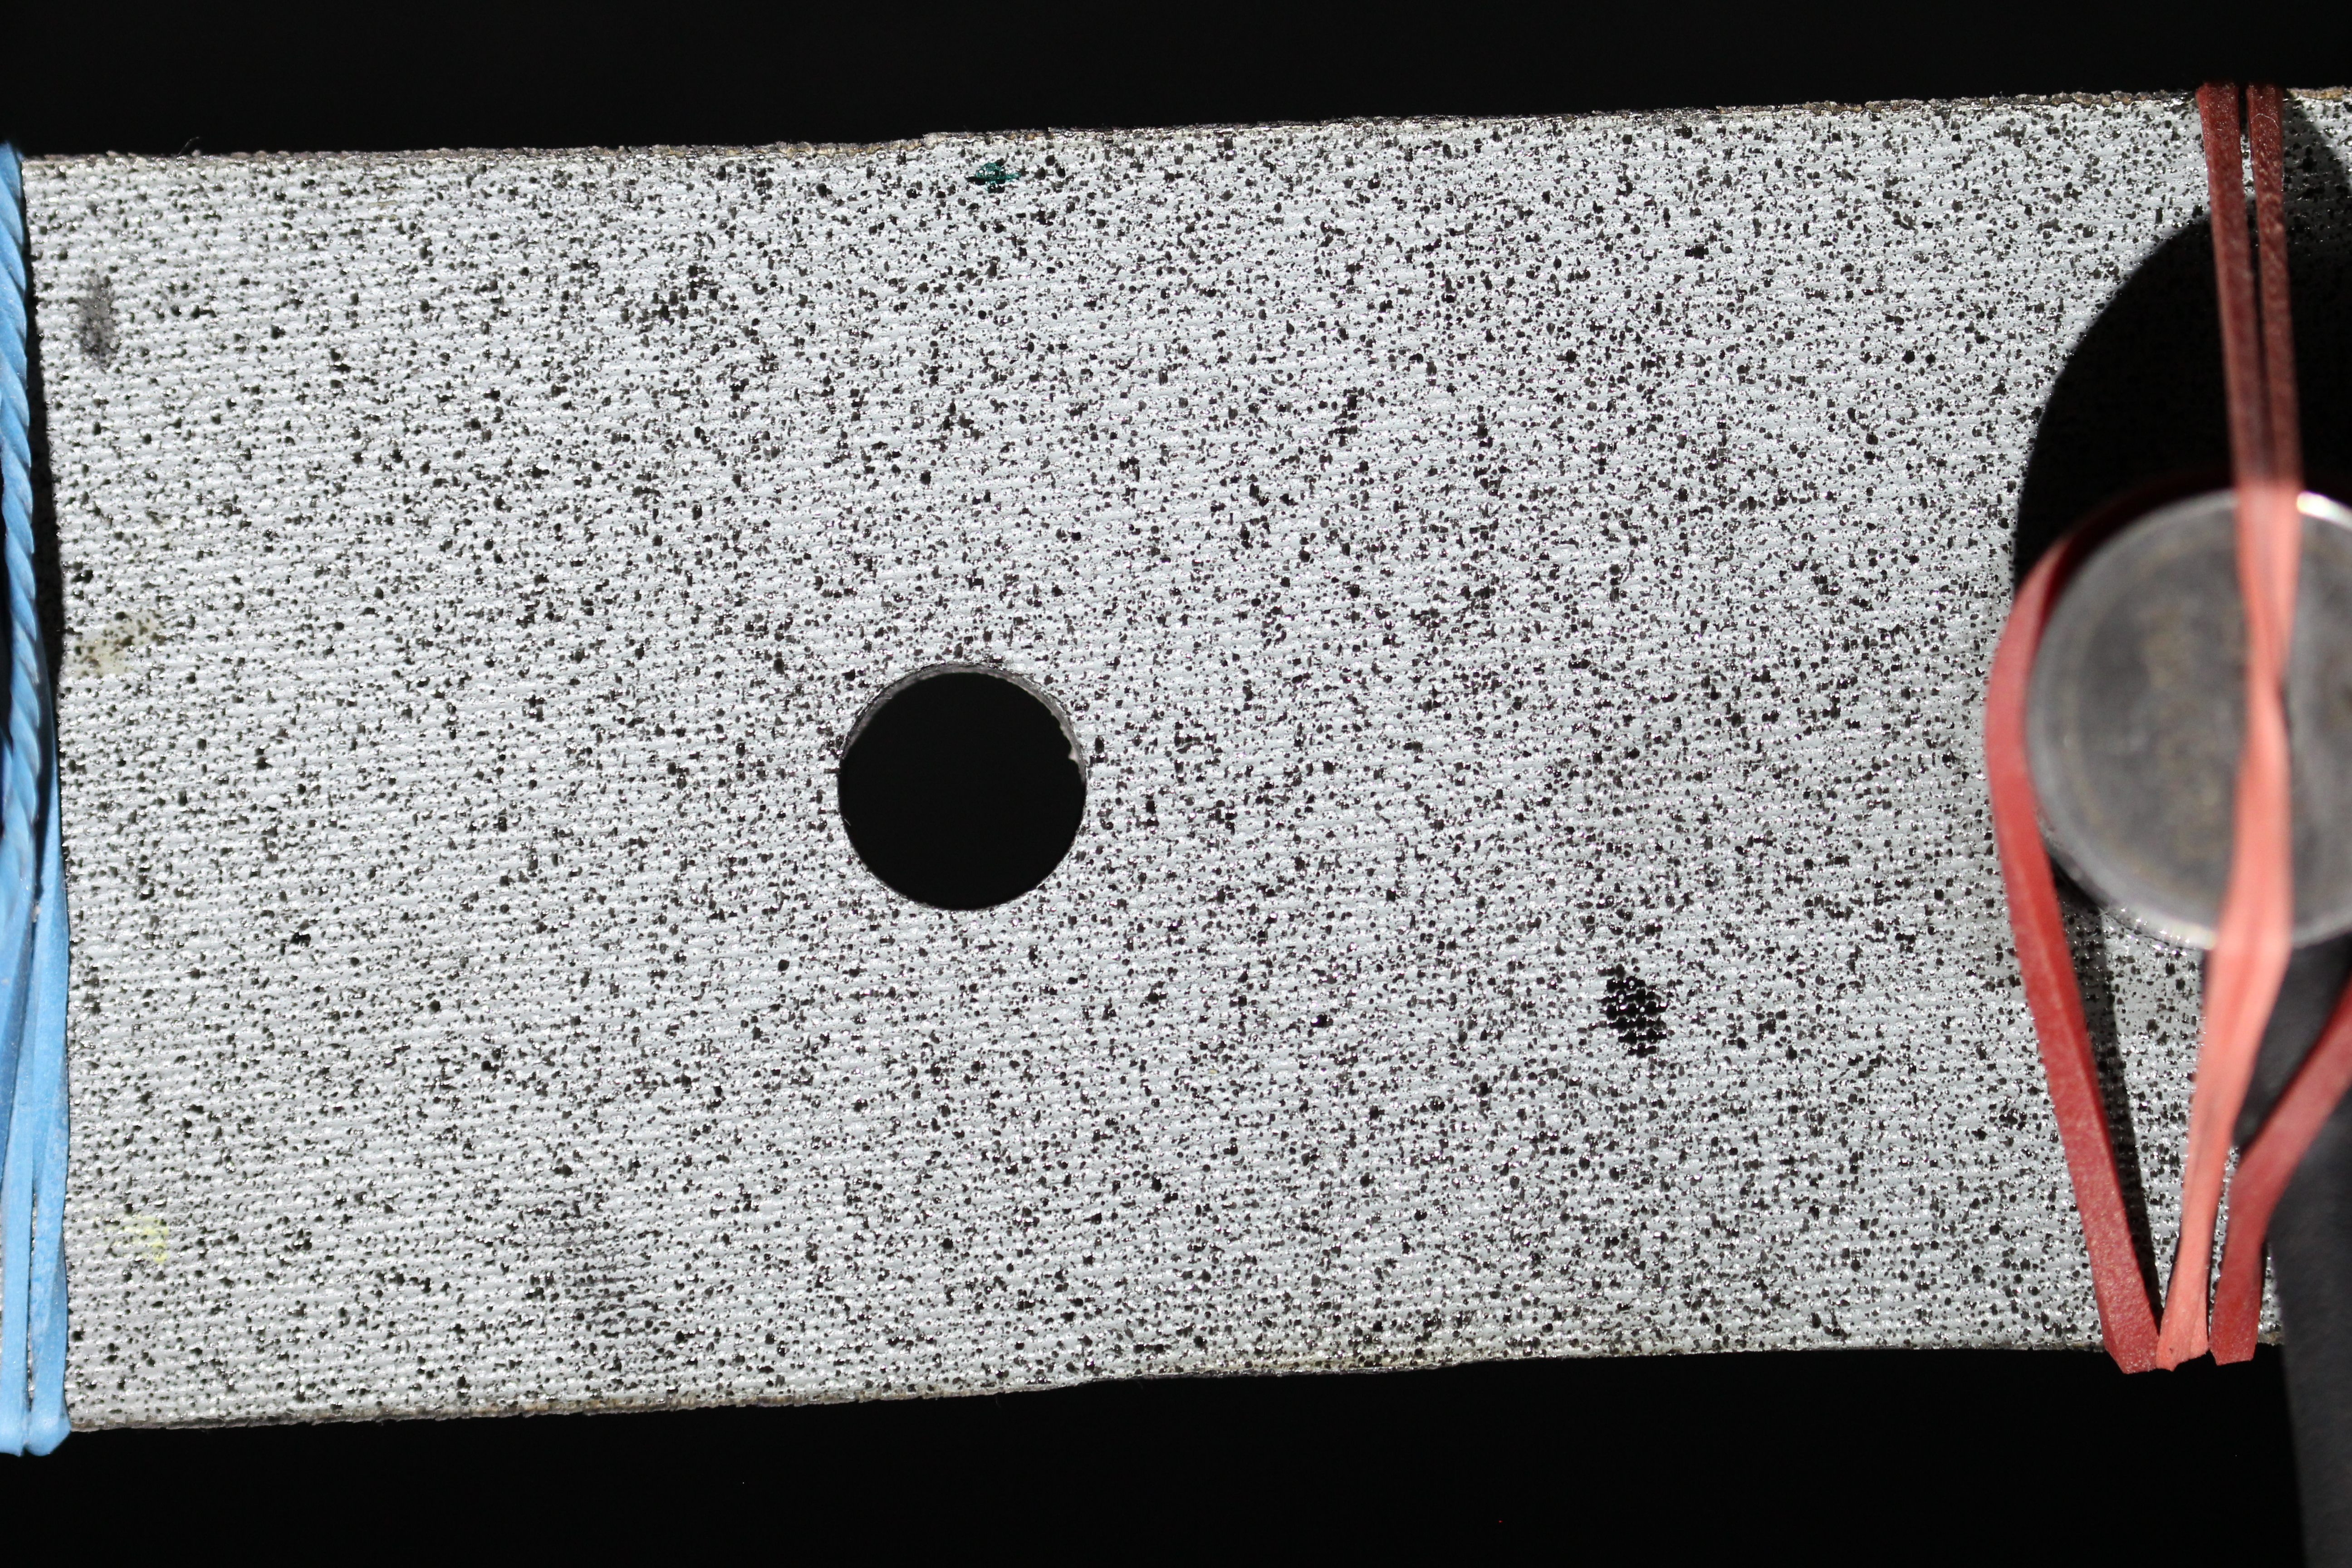
\includegraphics[width=0.6\linewidth]{carbon_deform}}
\caption{Углерод-углеродный композиционный материал}
\label{pic:carbon_deform}
\end{figure}

Фотографирование поверхности осуществляли с помощью фотокамеры Canon EOS 550D, оснащённой длиннофокусным объективом Canon EF-S 100-400mm 1/4-5.6 IS.

\subsection{Тестирование программного обеспечения}
\subsubsection{Тестирование на модельных изображениях}

Для первого раза используем изображения из серии Grey texture, представленные на рисунке \ref{pic:gray_set}. Они имеют сдвиг по оси $x$ на один пиксель влево, по $y$ сдвиг отсутствует.

\begin{figure}[ht]
\center{\includegraphics[width=0.6\linewidth]{gray_set}}
\caption{Тестовая серия изображений: Grey texture}
\label{pic:gray_set}
\end{figure}

Результатом работы ПО, как описано в первом разделе, является векторное поле и поля деформации твёрдого тела представленное на рисунке \ref{pic:gray_set_out}.

\begin{figure}[ht]
\center{\includegraphics[width=0.6\linewidth]{gray_set_out}}
\caption{Поле смещений и деформации твёрдого тела}
\label{pic:gray_set_out}
\end{figure}

\begin{figure}[ht]
\center{\includegraphics[width=0.6\linewidth]{gray_set_func_iteration}}
\caption{Зависимость уровня ошибки, от числа итераций}
\label{pic:gray_set_func_iteration}
\end{figure}

\begin{figure}[ht]
\center{\includegraphics[width=0.6\linewidth]{gray_set_func_iter_vector}}
\caption{Зависимость смещение по x, от числа итераций}
\label{pic:gray_set_func_iter_vector}
\end{figure}

\subsubsection{Тестирование на экспериментально полученных изображения}
В данном разделе приведены результаты тестирования разрабатываемого программного обеспечения на изображениях поверхностей реальных образцов.

\subsection{Исследование метода интерполяции}

\subsection{Исследование размера окна поиска}

\newpage
\section{Безопасность жизнедеятельности}
\subsection{Обоснование необходимости проводимого исследования}

\subsection{Планирование комплекса работ по разработке программного обеспечения}
Основными задачами планирования работ являются:
\begin{enumerate}
\item определение объема предстоящих;
\item распределение объема работ на взаимосвязанные последовательные этапы;
\item установление сроков выполнения работ;
\item определение необходимых, для выполнения планируемых работ денежных, материальных и трудовых ресурсов.
\end{enumerate}
При выполнении дипломной работы было задействовано два человека:
\begin{enumerate}
\item руководитель (рук.);
\item разработчик (разр.).
\end{enumerate}
Руководитель выполняет контроль выполнения различных этапов работ, согласованность этапов выполнения работ между собой, корректирует действия разработчика, дает рекомендации по выполнению тех или иных работ. Разработчик реализует тот объем работ, который установлен руководителем в соответствие с техническим заданием.

Месячный оклад студента в ТУСУР равен 1430 рублей, с учетом 21 рабочих дней в месяце, и 8 часового рабочего дня, стоимость одного часа работ равна 8,5 рублей. Месячный оклад руководителя д.н., профессора в университете равен 14800 рублей, с учетом 24 рабочих дней, и 6 часового рабочего дня, стоимость одного часа работ равна 102,8 рубля. [Приказ ректора от 22.03.2013 г. № 3106. С изменениями от 09.12.2013 г. № 14249]

График выполнения работ приведен в таблице 1.1.

Зная длительность цикла каждого этапа и возможность их параллельно-последовательного выполнения, можно рассчитать срок завершения планируемых работ и составить ленточный и сетевой графики плана их выполнения. Поскольку работа не требует большого состава исполнителей, то ограничимся ленточным графиком планирования, представленным в виде таблицы 1.2.

Таблица 1.2 – Ленточный график загрузки участников работ

\subsection{Определение сметной стоимости проекта}
\subsubsection{Общие положения}
Смета затрат для данной работы состоит из расходов, которые включают в себя следующие статьи:
\begin{enumerate}
\item затраты на оборудование и амортизацию;
\item расходы на оплату труда и отчисления на социальные нужды;
\item затраты на основные и вспомогательные материалы;
\item затраты на электроэнергию.
\end{enumerate}
\subsubsection{Затраты на оборудование и амортизацию}
Основным оборудованием при проведении работы являются компьютер и принтер, которые постановлением Правительства Российской Федерации от 1.01.02 г. N 1 отнесены ко второй амортизационной группе – «имущество со сроком полезного использования свыше 2 лет до 3 лет включительно». Месячная норма амортизации составляет 2,8\% и для компьютера, и для принтера.
Результаты расчетов амортизационных отчислений приведены в таблице 1.3.
Таблица 1.3 – Смета затрат на оборудование
\subsubsection{Расходы на оплату труда и отчисления на социальные нужды}
Статья затрат учитывает выплаты по заработной плате за выполненную работу, исчисленные на основании тарифных ставок и должностных окладов в соответствии с принятой в организации-разработчике системой оплаты труда. В этой статье также отражаются премии, надбавки и доплаты за условия труда, оплата ежегодных отпусков, выплата районного коэффициента и некоторые другие расходы. Отчисления на социальные нужды учитывают страховые взносы.
Результаты расчета расходов на оплату труда участников проекта представлены в таблице 1.4.
Таблица 1.4 – Расчет расходов на оплату труда участников проекта
\subsubsection{Затраты на основные и вспомогательные материалы}
Статья включает расходы по приобретению и доставке основных и вспомогательных материалов, необходимых для опытно-экспериментальной проработки решения, для изготовления макета или опытного оборудования. Сюда включаются и стоимость необходимых материалов для изготовления образцов и макетов, и материалов необходимых для оформления требуемой документации. 
Размер транспортно-заготовительных расходов (ТЗР), определяемый в процентах от стоимости, примем 10\%. Стоимость вспомогательных материалов принимается 10\% от стоимости основных материалов с учетом ТЗР. Результаты расчета стоимости материалов представлены в таблице 1.5.
Таблица 1.5 – Смета затрат на основные и вспомогательные материалы
\subsubsection{Расходы на электроэнергию}
Статья включает затраты по электроэнергии на технологические нужды. В настоящее время тариф на электроэнергию для населения г. Томска на 2015 год составляет 2,7 руб./ кВт ч. Введенный приказом от 26.12.2014 " №6/9 (691) ``О тарифах на электрическую энергию для населения и потребителей, приравненных к категории население по Томской области на 2015 год'', принятый департаментом тарифного регулирования Томской области.
Результаты расчетов приведены в таблице 1.6.
Таблица 1.6 – Затраты на электроэнергию
\subsubsection{Накладные расходы}
Расчет накладных расходов сведем в таблицу 1.7.
\subsubsection{Сводная смета затрат}
На основании всех произведенных расчетов составим сводную смету затрат на выполнение работы в виде таблицы \ref{tab:cmeta_zat}.

\begin{longtable}[h!]{|*2{m{0.5\textwidth}|}}
\caption{Сводная смета затрат}
\label{tab:cmeta_zat}
\hline
Наименование статей затрат                 & Всего, руб.       \\ \hline
ФОТ со страховыми взносами                 & 18442             \\ \hline
Основные и вспомогательные материалы       & 5478              \\ \hline
Амортизационные отчисления                 & 2520              \\ \hline
Затраты на электроэнергию                  & 983,88            \\ \hline
Накладные расходы                          & 720               \\ \hline
\multicolumn{2}{|l|}{Итого себестоимость работ: 36642,68 руб.} \\ \hline
\end{longtable}

\subsection{Научно-технический эффект}
Количественная оценка научно-технического уровня может быть произведена путем расчета результативности участников разработки по формуле:
\begin{equation}
K_{\text{ну}}=\sum (K_{de} \cdot d_i)
\end{equation}
где $$К\text{ну}$$ – коэффициент научного или научно-технического уровня;

$$К\text{ну}$$ – коэффициент научного или научно-технического уровня;

$$К\text{дуi}$$ – коэффициент достигнутого уровня i-го фактора;

$$di$$ – значимость i-го фактора;

$$n$$ – количество факторов.

$$К\text{дуi}$$ – коэффициент достигнутого уровня $$\text{i}$$-го фактора;

Весовые коэффициенты $d$ для каждого из факторов устанавливались экспертным путем. При этом сумма коэффициентов значимости по всем факторам равна единице. Коэффициенты достигнутого уровня факторов также установлены экспертным путем.

Рассчитанный коэффициент научно-технической результативности равен 0,7075. Полученное значение достаточно высоко, что говорит об эффективности проведенных работ выше среднего, однако отмечается необходимость дальнейшего развития проекта для достижения завершенности полученных результатов.

\subsection{Социальный эффект}
\newpage
\section{Технико-экономическое обоснование}
\subsection{Обоснование необходимости проводимого исследования}
Настоящая дипломная работа исследует алгоритмы поиска смещений по парам изображений основываясь на дифференциальном алгоритме Лукаса-Канаде. На основе полученных векторных полей смещений можно строить карты поверхностной деформации твердого тела.

Целью дипломной работы является разработка программного обеспечения (ПО) для оценки деформаций поверхностей твёрдых тел, а также проведение исследований алгоритмов и методов как на модельных, так и на реальных оптических изображениях.

\subsection{Планирование комплекса работ по разработке программного обеспечения}
Основными задачами планирования работ являются:

\begin{itemize}
\item определение объёма предстоящих работ;
\item распределение объёма работ на взаимосвязанные последовательные этапы;
\end{itemize}

\begin{itemize}
\item установление сроков выполнения работ;
\item определение необходимых, для выполнения планируемых работ денежных, материальных и трудовых ресурсов.
\end{itemize}
При выполнении дипломной работы было задействовано два человека:

\begin{itemize}
\item руководитель (рук.);
\item разработчик (разр.).
\end{itemize}

Руководитель выполняет контроль выполнения различных этапов работ, согласованность этапов выполнения работ между собой, корректирует действия разработчика, дает рекомендации по выполнению тех или иных работ. Разработчик реализует тот объем работ, который установлен руководителем в соответствие с техническим заданием.

Месячный оклад студента в ТУСУР равен 10483 рублей, с учетом 20 рабочих дней в месяце, и 8 часового рабочего дня, стоимость одного часа работ равна 65,51 рублей. Месячный оклад руководителя к.т.н., доцента в университете равен 14800 рублей, с учетом 24 рабочих дней, и 6 часового рабочего дня, стоимость одного часа работ равна 102,8 рубля.

График выполнения работ приведен в таблице \ref{tab:job_is_done_1}.

\begin{table}[!ht]
\caption{График выполнения работ}
\centering
\includegraphics[page=1, width=1\linewidth]{econom_table.pdf}
\label{tab:job_is_done_1}
\end{table}

Зная длительность цикла каждого этапа и возможность их параллельно-последовательного выполнения, можно рассчитать срок завершения планируемых работ и составить ленточный и сетевой графики плана их выполнения. Поскольку работа не требует большого состава исполнителей, то ограничимся ленточным графиком планирования, представленным в виде таблицы \ref{tab:eco_2}.

\begin{table}[!ht]
\caption{Ленточный график загрузки участников работ}
\centering
\includegraphics[page=2, width=1\linewidth]{econom_table.pdf}
\label{tab:eco_2}
\end{table}

\begin{table}[!ht]
\caption{Календарный график загрузки участников}
\centering
\includegraphics[page=3, width=1\linewidth]{econom_table.pdf}
\label{tab:eco_3}
\end{table}

\subsection{Определение сметной стоимости проекта}
\subsubsection{Общие положения}

Смета затрат для данной работы состоит из расходов, которые включают в себя следующие статьи:

\begin{itemize}
\item затраты на оборудование и амортизацию;
\item расходы на оплату труда и отчисления на социальные нужды;
\item затраты на основные и вспомогательные материалы;
\item затраты на электроэнергию.
\end{itemize}
\subsubsection{Затраты на оборудование и амортизацию}

Основным оборудованием при проведении работы являются компьютер и принтер, которые постановлением Правительства Российской Федерации от 1.01.02 г. N 1 отнесены ко второй амортизационной группе – «имущество со сроком полезного использования свыше 2 лет до 3 лет включительно». Месячная норма амортизации составляет 2,8\% и для компьютера, и для принтера.

Результаты расчётов амортизационных отчислений приведены в таблице \ref{tab:eco_4}.

\begin{table}[!ht]
\caption{Смета затрат на оборудование}
\centering
\includegraphics[page=4, width=1\linewidth]{econom_table.pdf}
\label{tab:eco_4}
\end{table}

\subsubsection{Расходы на оплату труда и отчисления на социальные нужды}

Статья затрат учитывает выплаты по заработной плате за выполненную работу, исчисленные на основании тарифных ставок и должностных окладов в соответствии с принятой в организации-разработчике системой оплаты труда. В этой статье также отражаются премии, надбавки и доплаты за условия труда, оплата ежегодных отпусков, выплата районного коэффициента и некоторые другие расходы. Отчисления на социальные нужды учитывают страховые взносы.

Результаты расчета расходов на оплату труда участников проекта представлены в таблице \ref{tab:eco_5}.

\begin{table}[!ht]
\caption{Расчет расходов на оплату труда участников проекта}
\centering
\includegraphics[page=5, width=1\linewidth]{econom_table.pdf}
\label{tab:eco_5}
\end{table}

\subsubsection{Затраты на основные и вспомогательные материалы}

Статья включает расходы по приобретению и доставке основных и вспомогательных материалов, необходимых для опытно-экспериментальной проработки решения, для изготовления макета или опытного оборудования. Сюда включаются и стоимость необходимых материалов для изготовления образцов и макетов, и материалов необходимых для оформления требуемой документации.

Размер транспортно-заготовительных расходов (ТЗР), определяемый в процентах от стоимости, примем 10\%. Стоимость вспомогательных материалов принимается 10\% от стоимости основных материалов с учетом ТЗР. Результаты расчёта стоимости материалов представлены в \ref{tab:eco_6}.

\begin{table}[!ht]
\caption{Расчёт затрат на основные и вспомогательные материалы}
\centering
\includegraphics[page=6, width=1\linewidth]{econom_table.pdf}
\label{tab:eco_6}
\end{table}

\subsubsection{Расходы на электроэнергию}

Статья включает затраты по электроэнергии на технологические нужды. В настоящее время тариф на электроэнергию для населения г. Томска на 2015 год составляет 2,7 руб./ кВт ч. Введенный приказом от 26.12.2014 {\textquotedbl} №6/9 (691) «О тарифах на электрическую энергию для населения и потребителей, приравненных к категории население по Томской области на 2015 год», принятый департаментом тарифного регулирования Томской области.

Результаты расчётов приведены в \ref{tab:eco_7}.

\begin{table}[!ht]
\caption{Затраты на электроэнергию}
\centering
\includegraphics[page=7, width=1\linewidth]{econom_table.pdf}
\label{tab:eco_7}
\end{table}

\subsubsection{Накладные расходы}

Расчет накладных расходов сведем в \ref{tab:eco_8}.

\begin{table}[!ht]
\caption{Накладные расходы}
\centering
\includegraphics[page=8, width=1\linewidth]{econom_table.pdf}
\label{tab:eco_8}
\end{table}

\subsubsection{Сводная смета затрат}

На основании всех произведённых расчётов составим сводную смету затрат на выполнение работы в виде таблицы \ref{tab:eco_9}.

\begin{table}[!ht]
\caption{Сводная смета затрат}
\centering
\includegraphics[page=9, width=1\linewidth]{econom_table.pdf}
\label{tab:eco_9}
\end{table}

\subsection{Научно-технический эффект}
Количественная оценка научно-технического уровня может быть произведена путем расчета результативности участников разработки по формуле:

{\centering\color{black}
 $\text{\textcyrillic{К}}_{\mathit{\text{\textcyrillic{н}}\text{\textcyrillic{у}}}}=\sum _{i=1}^n\left(\text{\textcyrillic{К}}_{\mathit{\text{\textcyrillic{д}}\text{\textcyrillic{у}}}}{\cdot}d_i\right)$,
\par}

где\ $K_\textit{ну}$ – коэффициент научного или научно-технического уровня;

%$K_\textit{ду}\textit{\textsubscript{i}}$ – коэффициент достигнутого уровня $\textit{i}{}$-го фактора;

%\textit{d}\textit{\textsubscript{i}}\textit{ }– значимость \textit{i}{}-го фактора;

\textit{n} – количество факторов.

Весовые коэффициенты \textit{d} для каждого из факторов устанавливались экспертным путем. При этом сумма коэффициентов значимости по всем факторам равна единице. Коэффициенты достигнутого уровня факторов также установлены экспертным путем.

\begin{table}[!ht]
\caption{Оценка научно-технического уровня разработки}
\centering
\includegraphics[page=10, width=1\linewidth]{econom_table.pdf}
\label{tab:eco_10}
\end{table}
Рассчитанный коэффициент научно-технической результативности равен 0,7075. Полученное значение достаточно высоко, что говорит об эффективности проведенных работ выше среднего, однако отмечается необходимость дальнейшего развития проекта для достижения завершенности полученных результатов.

\subsection{1.5 Социальный эффект}
Гипотетический социальный эффект заключается в улучшении результатов исследований, проводимых в лаборатории механики полимерных композиционных материалов СО РАН, которые могут использовать программное обеспечение оценки деформации твердых тел, и усилении научного потенциала.
\newpage
\section{Заключение}
\setcounter{figure}{0}

В результате выполнения работы было разработано программное обеспечение для оценки деформаций поверхности твёрдого тела.  ПО позволяет оценивать оптический поток по серии входных снимков и проводить исследования механизмов пластической деформации на мезоуровне. %Основная отличительная особенность ПО от разработок существовавших ранее в том, что оно позволяет производить расчеты от качественных показателей (ПВС) до количественных результатов в виде компонент деформации с возможностью корректировки промежуточных результатов. Таким образом, ПО объединяет в себе средства для решения нескольких задач. 

При разработке ПО были рассмотрены и реализованы методы вычисления оптического потока на основе алгоритма Лукаса-Канаде, его пирамидальная версия, и итеративная модификация с субпиксельной точностью.

Экспериментальное исследование алгоритмов определения ПВС показало, что при уровне использующейся в настоящее время вычислительной техники наиболее эффективен корреляционный алгоритм с заданием области расчета коэффициента корреляции, т.к. это наиболее точный метод (из реализованных в ПО) при приемлемых вычислительных затратах. Алгоритмы, оптимизированные по времени расчета, могут использоваться для быстрой предварительной оценки ПВС.
Предложенный алгоритм нахождения ПВС с субпиксельной точностью показал свою эффективность при расчете компонент тензора дисторсии. Повышение точности определения векторов смещений до долей пиксела позволяет более точно и корректно рассчитать распределения компонент деформации.
\newpage
\renewcommand{\refname}{Список использованных источников}
\bibliography{lib}
\ESKDappendix{обязательное}{\normalfont Текст графического модуля}
\begin{lstlisting}
import QtQuick 2.4
import QtQuick.Controls 1.3
Item {
    width: 400
    height: 240
    ComboBox {
        id: comboBox1
        x: 150
        y: 0
        model: [ "B-spline", "Bilinear", "Bicubic" ]
    }   
    Label {
        id: countInterpolation
        x: 20
        y: 5
        text: qsTr("Interpolation")
    } 
    SpinBox {
        id: countIteration
        x: 150
        y: 40
        minimumValue : 1
        maximumValue : 100
        value : 10
    }
    SpinBox {
        id: windowSearch
        x: 150
        y: 80
        minimumValue : 2
        maximumValue : 1000
        value : 16
    }
    SpinBox {
        id: stepGrid
        x: 150
        y: 120
        minimumValue : 1
        maximumValue : 500
        value : 16
    }
    Label {
        id: countIterationLabel
        x: 20
        y: 40
        text: qsTr("Count iteration")
    }
    Label {
        id: labelWindowSearch
        x: 20
        y: 80
        text: qsTr("Size window search")
    }
    Label {
        id: labelStepGrid
        x: 20
        y: 120
        text: qsTr("Step for grid")
    }
    TextField {
        id: outDirField
        objectName: "outDirField"
        x: 20
        y: 160
        placeholderText: qsTr("Output directory")
    }
    Button {
        id: buttonOutDirField
        x: 150
        y: 160
        text: qsTr("Browse")
    }
    CheckBox {
        id: debugCheckBox
        x: 20
        y: 200
        text: qsTr("More log")
        checked: false
    }
    CheckBox {
        id: pyramidCheckBox
        x: 150
        y: 200
        text: qsTr("Use pyramid")
        checked: true
    }
    function getcmd()
    {
      return "lucas_kanade";
    }
    function getarg()
    {
      var a = 
      [
        "-l", outDirField.text + "/list",//load list image
        "-o", outDirField.text,//output directory
        "-i", countIteration.value,//count iteration (1 by default)
        "-w", windowSearch.value,//size window search (3px by default)
        "-g", stepGrid.value,//step for grid (5px by default)
        "-b", comboBox1.currentIndex,
        pyramidCheckBox.checked ? "-p" : "",
        debugCheckBox.checked ? "-d" : "",
        /*"-h", //show help
        "-v" //show version*/
      ];
      return a;
    }
    function outdir() 
    {
      return outDirField.text;
    }
}
\end{lstlisting}
\ESKDappendix{обязательное}{\normalfont Документация программного обеспечения}
\vspace*{7cm}
\begin{center}%
\LARGE {Lucas Kanade}\\\large{1.4}\\
\vspace*{1cm}
{\large Создано системой Doxygen 1.8.9.1}\\
\vspace*{0.5cm}
{\small Пт 5 Июн 2015 02:43:45}\\
\end{center}
\includepdf[pages={2-}]{refman.pdf}
\end{document}